\documentclass[a4paper]{article}

\usepackage[english]{babel}
\usepackage[utf8x]{inputenc}
\usepackage{amsmath}
\usepackage{float}
\usepackage{subcaption}
\usepackage{graphicx}
\usepackage[authoryear]{natbib}
\usepackage{hyperref}
\usepackage{booktabs}
\usepackage[margin=1in]{geometry}
\usepackage{pgfplots}
\usepackage{siunitx,etoolbox}
\pgfplotsset{compat=1.12}

\sisetup{
  table-align-uncertainty=true,
  separate-uncertainty=true,
}
%% local redefinitions
\renewrobustcmd{\bfseries}{\fontseries{b}\selectfont}
\renewrobustcmd{\boldmath}{}

\title{Enhancing Competitive Intelligence Acquisition Through Embeddings and Visual Analytics}
\author{David Silva, Fernando Bação}
\date{}

\begin{document} 
\maketitle

\begin{abstract}
	Briefly summarize your previous work, goals and objectives, what you have accomplished, and future work. (100 words max) If you have a question, please use the help menu (''?'') on the top bar to search for help or ask us a question.
\end{abstract}

\section{Introduction}
% Introducing the topic: Opening with a strong opening hook
Competitive Intelligence (CI) is the process and forward-looking practices used in producing knowledge about the competitive environment to improve organizational performance \citet{madureira2021}. According to \citet{brod1999}, "Companies with competitive intelligence programs have better knowledge of their markets, better cross-functional relationships between their business units and a greater ability to develop proactive competitive strategies." CI has a fundamental role in helping businesses remain competitive, influencing a wide range of decision-making areas, and leading to substantial improvements such as the increase of revenue, new products or services, cost savings, time savings, profit increases, and achievement of financial goals \citep{calof2017}.

% Making the case and defining the goal of the paper
Competitive Intelligence analysts are responsible for developing the CI task through a combination of gathering data, processing it, and communicating information. The digitalization of the market and the growth of the data economy have pushed the business environment to an online realm where every action and event is public and thus potentially relevant for decision-making. This shift has produced a large volume of data about products, customers, competitors, and any aspect of the business environment that can be used to foresee opportunities and risks. Given the vastness and diversity of this data, it has become a necessity to design tools that can aid analysts in the CI gathering and analysis process. Therefore, the goal is to enhance the analyst's task by providing a tool to explore, organize and visualize the environmental data present in the array of existing sources.

Traditionally, the most important sources of CI have been, respectively, news providers, corporate websites, and trade publications \citep{marin2004}. With the advent of the internet, new sources, such as social networks \citet{dey2011}, have emerged, while existing ones have become enriched and easily accessible. Despite the increased availability, CI resources are dispersed through a variety of websites and the underlying data is unstructured and noisy. These characteristics add to the difficulty of the analyst's task and exacerbate the need for tools to support it.

% Describe the background: an overview of the most relevant research that has already been conducted (what has been done and what are the limitations that we intend to explore)
Various studies have attempted to create systems for exploring and gathering intelligence from large collections of textual data \citep{dey2011, esteva2020, lafia2019, lafia2021a}. These studies have consistently applied Natural Language Processing (NLP) techniques for helping users comprehend large volumes of text without requiring to sift through every document. \citet{dey2011} designs a system for CI that captures data from multiple sources, cleans it, uses NLP to identify and tag the relevant content, stores it, generates consolidated reports, and produces alerts on pre-defined triggers.

% Establish your research problem: clarify how your own research fits in and what problem it addresses
% TODO: SHOULD WE TALK ABOUT INFORMATION ENCOUNTERING ANYWHERE ELSE IN THE PAPER?
Although the previously mentioned systems have successfully been used for dealing with large amounts of text, insufficient attention has been paid to the exploratory and serendipitous aspects of the analyst's task. Accordingly, we propose an information environment that supports analysts in having stimulating and productive information encounters. Thus, contrarily to previous systems, we center ours around Information Encountering which is defined by \citet{erdelez2020} to encompass "finding interesting, useful or potentially useful information when looking for some other information, not looking for any information in particular, or not looking for information at all". This is achieved by incorporating two types of information acquisition tasks: \emph{searching}, consisting of an information retrieval module that allows ad hoc queries on the entire document collection, giving the user the ability to actively seek information, and \emph{browsing}, consisting of a visualization module that equips the user with tools to actively or passively acquire information through the visual exploration of the document corpus (and its thematic cohorts) in a two-dimensional map. 

% Talk about the recent advent of the transformers as a justification for this system and as a distinguishing factor
Another unique characteristic of our work is the use of state-of-the-art NLP techniques. With the recent emergence of the Transformer architecture \citep{vaswani2017}, significant improvements were made in several NLP subdomains. This new architecture is based solely on the attention mechanism, providing parallelization capabilities and significant improvements in training time. Also, the Transformer can more easily learn long-range relationships between terms in the input sequence than pre-existing architectures \citep{vaswani2017}. Language models like Bidirectional Encoder Representations from Transformers (BERT) \citep{devlin2019} leverage this architecture, making up a large part of the modern NLP landscape by providing an off-the-shelf, powerful way to create state-of-the-art models for a wide range of tasks.

% Specify your objective(s): what you intend to find out or express in your paper
In this paper, we explore Transformer-based models for representing documents as semantic vectors. These vectorial representations are commonly denominated as embeddings and we intend to use them in a CI system as a mechanism for extracting information from environmental data. Furthermore, the system facilitates Information Encountering by incorporating searching and browsing mechanisms that leverage the document embeddings.

\section{Related Work}
% Introduction: The introduction should clearly establish the focus and purpose of the literature review.
The process of extracting business-related information for anticipating risks and opportunities is an important task for many companies, yet analysts are overwhelmed with large amounts of unstructured data. To support CI analysts, we propose an NLP system for exploring and gathering intelligence from large collections of textual data. To situate our contribution, we review, in this section, existing work in similar systems applied in CI as well as in other domains.

% Body: Summarize and synthesize, Analyze and interpret, Critically evaluate, write in well-structured paragraphs
Early work on visualizing and interpreting large collections of documents can be found in \citet{kaski1998}, where WEBSOM - a system that organizes a document collection using Self Organizing Maps (SOM) \citep{Kohonen1982}, mapping each document into the node of a two-dimensional grid that best represents it, thus providing a reliable and visual representation of the collection - is presented. An improved version of the system is given in \citet{kohonen2013}, where users can perform queries using either a set of keywords or a descriptive sentence, a zooming feature to explore specific regions of the map with finer detail is provided and, when selecting a particular node in the map, the titles of the corresponding documents are displayed. \citet{lafia2019} also uses SOM together with Latent Dirichlet Allocation (LDA) \citep{blei2003} to convey the relatedness of research themes in a multidisciplinary university library. Documents are represented as random mixtures over latent topics, where each topic is characterized by a distribution over words. That said, each document is embedded in a vector space of \emph{n} dimensions, corresponding to the number of topics selected. SOM produces a landscape for exploring the topic space and provides users with an overview of the document collection and the ability to navigate, discover items of interest, change the level of detail, select individual documents and discover relationships between documents.

Arguably, the closest system to ours in terms of domain application is \citet{dey2011}. They formulate a system for acquiring competitive intelligence from different types of web resources, including social media, using a wide array of text mining techniques. They also show how the system can be integrated with the business data and adopted for future decision-making. Their goal is to help the analyst in the task of reading, extracting information, and organizing the data. The system is composed of four distinct modules: \emph{content acquisition and assimilation} gathers and extracts relevant content from an array of sources, \emph{data pre-processing} is responsible for cleaning and extracting relevant content from different sources, \emph{content processing} identifies and tags the relevant content from the vast collection, and \emph{alerting} notifies the user on pre-defined triggers such as competitor's product launch. The paper presents an approach for labeling news articles according to CI-related topics by applying LDA clustering and extracting entities and relations within each cluster, which are then used to define the respective labels. The labeling contributes to the organization of the collection and facilitates the information extraction process.

\citep{lafia2021a} proposes a method for modeling and mapping topics from bibliometric data and builds a web application based on this method. The map produced allows users to read a body of research "at a distance" while providing multiple levels of detail of the documents' topics. They also incorporate a time dimension, allowing users to understand the evolution of the topics over time. They apply Non-negative Matrix Factorization \citep{lee1999} to discover the underlying topics in the data and obtain vectorial representations of the documents, and they employ t-distributed Stochastic Neighbor Embedding (t-SNE) \citep{vandermaaten2008} for visualizing the documents, resulting in a two-dimensional representation of the corpus. To allow for different detail levels, the authors produce two maps: a coarse map of 9 topics that gives a general overview of the topics within the data and a detailed map of 36 topics that captures more specific research themes. The web application consists of an interactive dashboard that allows users to explore the map of documents and easily extract information.

The Vector Space Model (VSM) \citep[p.~120-126]{schutze2008} is a common framework in Information Retrieval, consisting of representing a set of documents as vectors in a vector space, while also allowing full-text queries to be represented in the same space. The model then ranks each document in decreasing order of their similarity with the query. The fundamental assumption of the model is that similar documents will be placed close together in the vector space, whereas dissimilar documents will be far away. An application of VSM for medical imaging can be found in \citep{sampathila2020}. They propose a methodology for Content-based Medical Image Retrieval where Magnetic Resonance Imaging (MRI) images are represented using features such as color, shape, and texture, and the \emph{k} items with the smallest euclidean distance to a given query image are retrieved. They report that by using this approach they can classify dementia-affected MRI images with an average precision of 97.5\% and a maximum recall of 95\%, making it an effective way to diagnose new images. \citep{esteva2020} presents a different application of VSM for querying COVID-19 literature. They propose Co-Search, an Information Retrieval system that combines semantic search, question answering, and abstractive summarization. The system uses Sentence-BERT (SBERT) \citep{reimers2019}, a Transformer-based model for representing documents as semantic vectors, combining it with approximate nearest neighbors and cosine similarity to return the relevant results for a query.

% Conclusion: summarize the key findings you have taken from the literature and emphasize their significance - is this necessary?

% Describe what was done, how it was done, and justify the experimental design. Enough detail to reproduce and judge the results.
% TODO: Support the claims below (scalable, dynamic and fast) in results!
\section{Method}
We propose a system — Figure \ref{system_architecture} — that supports the exploration of a document collection while promoting serendipity and can satisfy emerging information needs by allowing full-text queries over the entire collection.
The system is scalable to large amounts of data, is dynamic as it regularly integrates new data, and is fast. It is composed of three main pipelines: Indexing, Query, and Visualization which objectives are respectively, to get documents and their metadata from a source to a database, to retrieve the most relevant results to a user query, and to produce an interactive interface for exploring the document collection. The code developed for this work can be accessed at \href{https://github.com/DavidSilva98/mapintel_project}{github.com/DavidSilva98/mapintel\_project}.

\begin{figure}[H]
	\centering
	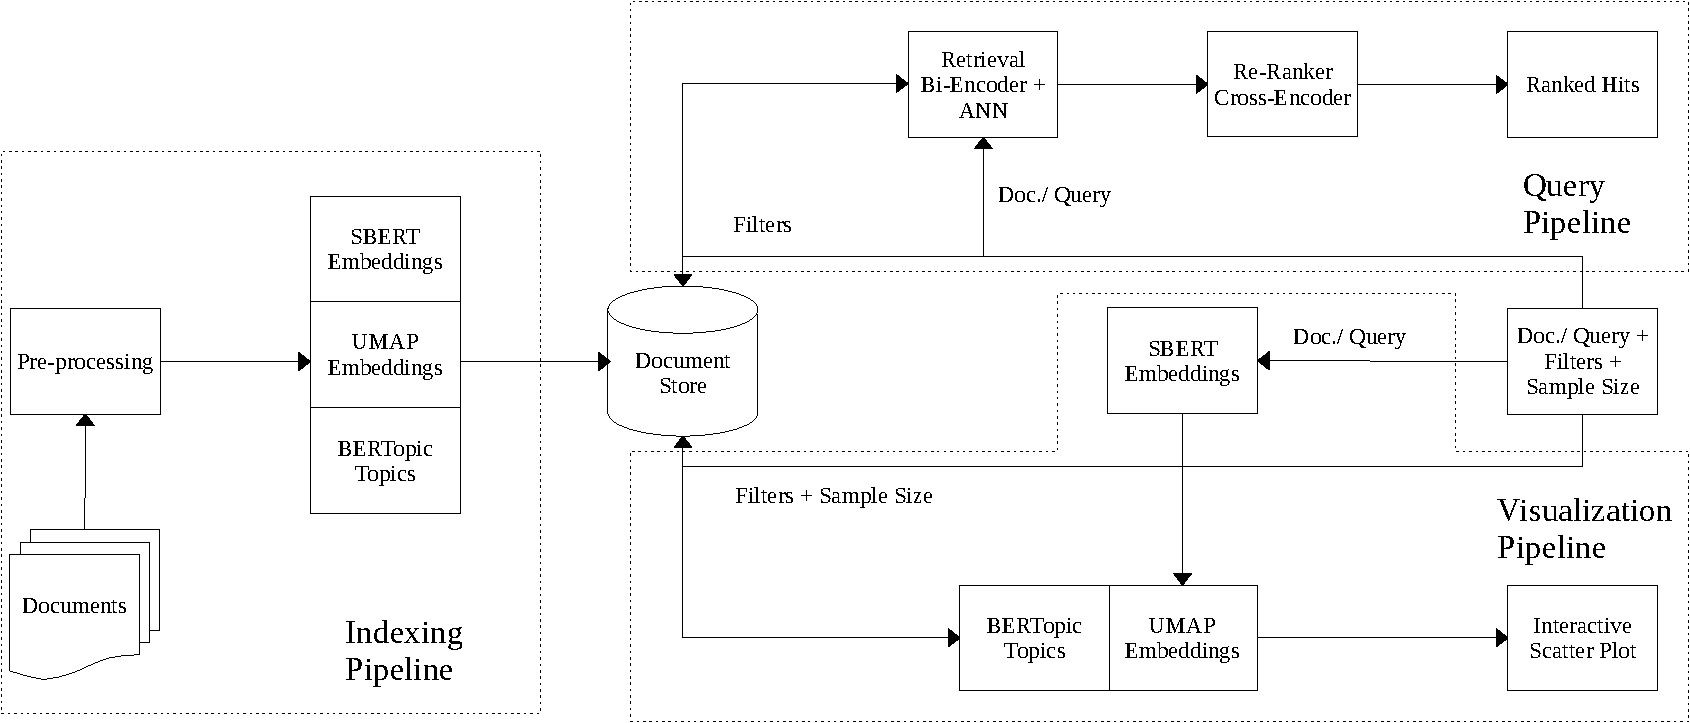
\includegraphics[scale=0.5]{./assets/system_architecture}
	\caption{System Architecture}
	\label{system_architecture}
\end{figure}

\subsection{Indexing} \label{indexing}
In this work we decided to focus on how NLP and particularly sentence embeddings could help in organizing, exploring, and retrieving text documents in the CI domain. As already stated, there are multiple sources of CI, and different information can be obtained from these. \citet{dey2011} shows in Table \ref{table1} what kind of information can be acquired from these sources, particularly the ones that are easily available through the web. We decided to work mainly with news articles as they provide a general and accessible means of information about the environment, however, our methodology is easily extensible to data from different sources and can be applied in various settings. 

% Is it ok to put this table from another paper here in the way it is presented?
\begin{table}[]
  \centering
  \resizebox{\textwidth}{!}{%
    \begin{tabular}{@{}ll@{}}
      \toprule
      \textbf{Type of Competitive Intelligence}          & \textbf{Web Resources}                             \\ \midrule
      People event                                       & News, company web-sites                            \\
      Competitor strategies, Technology investment, etc. & News, Discussion forum, Blogs, Patent search sites \\
      Consumer sentiments                                & Review sites, Social networking sites              \\
      Promotional events and pricing                     & Social networking sites                            \\
      Related real-world events                          & News, Social networking sites                      \\ \bottomrule
    \end{tabular}%
  }
  \caption{Competitive Intelligence resources on the web - \citet{dey2011}}
  \label{table1}
\end{table}

To obtain news articles from multiple international sources, we use a REST API\footnote{\href{https://newsapi.org/}{newsapi.org}}. The API retrieves the articles, as well as their metadata, consisting of attributes such as source, author, title, description, content, category, URL, and publication date and time. We use this API to feed the system with updated data on a schedule while focusing on articles written in English from a set of predefined categories (business, entertainment, general, health, science, sports, technology).

Due to API limitations, the retrieved data has its content attribute truncated to 200 characters. To overcome this, we treat a single document unit as the concatenation of title, description, and content, providing us a semantically loaded piece of text that we can use for NLP purposes. Despite this limitation, we give the user the possibility of accessing the full article through its URL. We ensure that each document is unique, is written in English, and doesn't have any HTML tags or any strange pattern.

After, we produce the embeddings of each document. This process is the basis of our work as it allows us to encode the semantic identity of the article onto a vector of a given dimensionality. This semantic identity describes what is the subject of the article, and it can be used to compare documents between each other i.e. articles with the same subject will be close in the semantic space and vice-versa. We use SBERT \citep{reimers2019}, a derivative of the Transformer-based BERT model, to embed the documents using a pre-trained encoder trained on reducing the distance between queries and relevant results in the MS MARCO dataset \citep{bajaj2018}. This produces vectors of 768 dimensions, which we then reduce to 2 dimensions using the Uniform Manifold Approximation and Projection (UMAP) \citep{mcinnes2020} algorithm. UMAP constructs a topological representation of the high and low dimensional data and its goal is to minimize their cross-entropy, which measures the difference between the two representations, by adjusting the low-dimensional representation. This is another important component of our system as it allows the organization and localization of the entire document collection in a 2-dimensional map, which can be used to explore and interact with the data. We opted to use UMAP over other dimensionality reduction techniques because of its improved map quality, reduction in time required to produce the output map, support for larger data set sizes, and, most importantly, its ability to update the output map with new data without having to rebuild it \citep{mcinnes2020}.

% Write about the best topic modeling technique we end up using and in the Results, we do the comparison.
We also apply a topic modeling technique called BERTopic \citep{grootendorst2020}, based on the work of \citet{angelov2020}. Topic modeling unveils the latent semantic structure of the data and unlike some of the classical techniques such as Latent Dirichlet Allocation \citep{blei2003} and Probabilistic Latent Semantic Indexing \citet{hofmann1999}, BERTopic leverages the SBERT embeddings and their capacity to encode the semantic attributes of a document to find the most representative topics of a corpus. BERTopic clusters the documents using Hierarchical Density-Based Spatial Clustering of Applications with Noise (HDBSCAN) \citep{mcinnes2017} to find the densest areas of the semantic space while identifying outliers. To overcome the sparsity of the high-dimensional space and the obstacles it creates in finding dense clusters, UMAP is used to reduce the embeddings to a lower dimension (5 dimensions by default) prior to the clustering stage. The main assumption behind BERTopic is that each dense area in the semantic space is generated by a latent topic shared among the documents that comprise it. Finally, a class-based variant of TF-IDF \citep{jones1972} (c-TF-IDF) is used to extract for each cluster an importance value of each word, which can be used to represent each topic as the set of its most important words. Another advantage of BERTopic over the classical approaches is that we can reduce the number of topics obtained by iteratively comparing the c-TF-IDF vectors, merging the least common topic with its most similar topic, and re-calculate the c-TF-IDF vectors, giving us the option to choose the number of topics.

Finally, we load the documents, their metadata, their SBERT embeddings, their UMAP embeddings, and their topics into a database. We use Open Distro for Elasticsearch\footnote{\href{https://opendistro.github.io/for-elasticsearch/}{opendistro.github.io/for-elasticsearch}} — an open-source, RESTful, distributed search and analytics engine based on Apache Lucene\footnote{\href{https://lucene.apache.org/}{lucene.apache.org}} — to store the data, organize it in an index and perform full-text search on it. We can think of the approach described as an Indexing Pipeline — Figure \ref{indexing_pipeline} — that extracts new raw documents from a data source, pre-processes and manipulates them, stores the results in a database, and indexes the documents for future search tasks.

\begin{figure}[H]
	\centering
	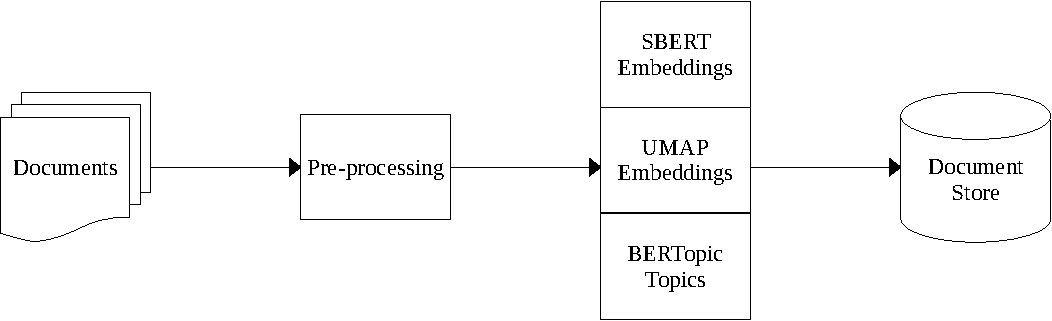
\includegraphics[scale=0.7]{./assets/indexing_pipeline}
	\caption{Indexing Pipeline}
	\label{indexing_pipeline}
\end{figure}

\subsection{Query}
Finding meaningful information within a large amount of data is a big part of the CI task. The ability to retrieve relevant documents from a large collection of news articles through natural language queries empowers the CI analyst with an easy and intuitive interface to scan the environment.

Our system provides a search functionality based on Open Distro for Elasticsearch and its k-Nearest Neighbor (k-NN) Search module. By utilizing the k-NN module, we can leverage the SBERT embeddings by projecting the query string onto the same semantic space as the corpus and computing its k-nearest neighbors i.e. finding the k documents whose embedding vectors are closest to the query embedding vector, according to some pre-defined similarity metric. Since the embedding vectors encode the semantic identity of each document, this method provides semantically relevant results for a given query. Furthermore, the k-NN module delivers a highly performant and scalable similarity search engine by leveraging Elasticsearch’s distributed architecture and by implementing Approximate Nearest Neighbors (ANN) search based on Hierarchical Navigable Small World Graphs \citep{malkov2018}. The k-NN module can also be combined with binary filters that help the user obtain focused results based on characteristics of the documents such as publication date and topic. These filters are applied directly to the database, reducing the search space as a result and improving the subsequent search time.

Once again, we can think of the search functionality as a pipeline, illustrated in Figure \ref{query_pipeline}, where we feed a query string and some binary filters, and we obtain documents ordered by their relevancy to the query. We employ a Retrieve and Re-rank pipeline based on the work of \citet{nogueira2020a, kratzwald2019} composed by a "Retrieval Bi-Encoder + ANN" node that performs semantic search using Elasticsearch’s k-NN module as described above, and by a "Re-Ranker Cross-Encoder" node consisting of a BERT model fine-tuned on the MS MARCO dataset that receives a document and query pair as input and predicts the probability of the document being relevant to the query. 

The pipeline works by taking advantage of the characteristics of both nodes. The Bi-Encoder together with ANN search can retrieve fairly relevant candidates while dealing efficiently with a large collection of documents. The Cross-Encoder isn't as efficient since it has to be performed independently for each document, given a query. However, since attention is performed across the query and the document, the performance is higher in the second node \citep{humeau2019}. Therefore, we combine both nodes by retrieving a large set of candidates from the entire collection using the Bi-Encoder, and by filtering the most relevant candidates with the Cross-Encoder while removing noisy results.

With this pipeline, we can provide relevant documents to the user given a query and binary filters while ranking them according to a relevancy score. The pipeline is efficient and makes use of the SBERT embeddings and the Elasticsearch architecture. As an additional feature, we can input a document instead of a query, allowing us to search for semantically similar documents within the collection.

\begin{figure}[H]
	\centering
	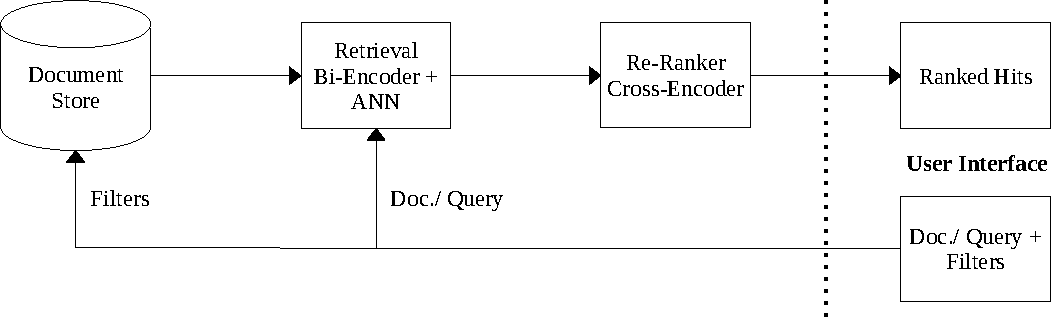
\includegraphics[scale=0.7]{./assets/query_pipeline}
	\caption{Query Pipeline}
	\label{query_pipeline}
\end{figure}

\subsection{Visualization}
To facilitate the environment scanning task, we developed a visual interface that organizes and displays the news articles, giving the user the ability to browse the data and zoom on particular regions of the semantic space. The interface uses the UMAP algorithm to reduce the dimensionality of the original semantic space to a 2-dimensional representation that reliably preserves the original topology.

The methodology employed to produce the interface is described in Figure \ref{vis_pipeline}. It begins by taking the same inputs passed to the Query pipeline: a query, and a set of filters. The common inputs create a connection between the two modules — when the user queries the database, the query text is projected onto the 2-dimensional map and the filters define which points are displayed in the map. In this way, the map can be seen as a graphical extension of the searching mechanism, where the relevant results reside in the neighborhood of the query, giving the user some insight into how the results are obtained. In addition to the common inputs, we require a relative sample size that defines the percentage of randomly chosen documents (after applying the filters) to be displayed in the map. This is necessary as interaction with the map is hindered by a large number of data points, resulting in a slow and unresponsive experience. Notice that the sample size doesn't affect the query results, as the search is always performed on the entire collection.

To produce the interactive scatter plot, the filters and sample size are used to select the documents to be displayed from the database. We compute the SBERT embedding of the query, followed by its UMAP embedding, thus being able to locate the query in the same space as the documents. An advantage of these two models is that we can efficiently produce embeddings of new text without having to re-train them, making this process quite fast. Once we have the UMAP embedding of the query, we join it with the pre-computed embeddings of the documents from the Indexing pipeline, and we produce the interactive map.

The map provides a means to explore the news articles and the different semantic cohorts present within the collection. We color-code the points with the documents' topics identified in the Indexing stage, allowing us to visualize the latent semantic structure of the data, and when hovered, the points display their corresponding title and content attributes.

\begin{figure}[H]
	\centering
	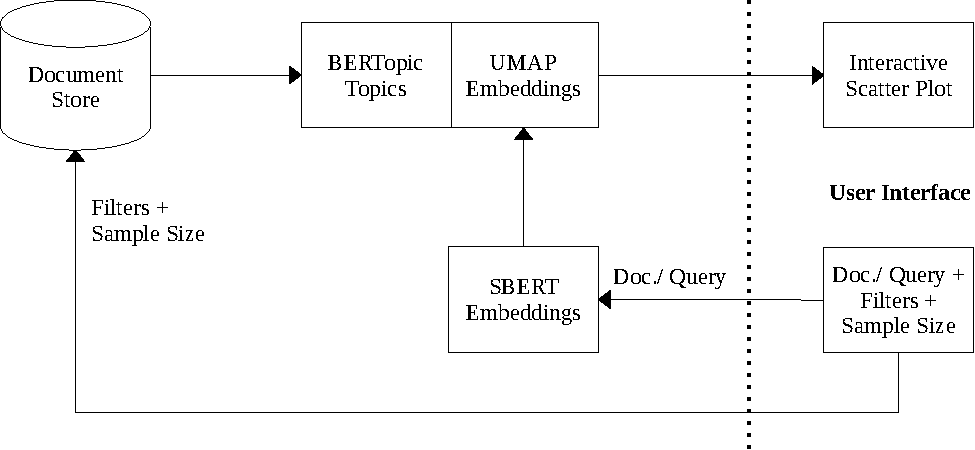
\includegraphics[scale=0.7]{./assets/vis_pipeline}
	\caption{Visualization Pipeline}
	\label{vis_pipeline}
\end{figure}

\section{Evaluation}
% Take a look at CO-Search,(especially this one. Just copyt the same format) DPR and Lafia 2021 paper for inspiration
Our methodology addresses the issues of information dispersion and overload impacting the CI analysts' task. The proposed system provides searching and browsing capabilities, contributing to an easier understanding of the business environment by supporting analysts in seeking specific information, while promoting undirected information encoutering. In this section, we fundament our choices in the design of the system with experiments and analyse the different components of the system individually.

\subsection{Experimental Setup}
We evaluate our system quantitatively using the 20 newsgroups \citep{pedregosa2011} dataset and the document labels provided. This dataset consists of around 18,000 newsgroups posts on 20 topics divided into 6 main groups: "Computer", "Recreation", "Science", "Miscellaneous", "Politics" and "Religion".

The following algorithms are compared in our paper:
\begin{itemize}
  \item \textbf{Sentence embeddings}
    \begin{enumerate}
      \item \textbf{Paragraph Vector Model (or Doc2Vec)} \citep{le2014}: an unsupervised algorithm that learns both word and document vectors by minimizing the error of predicting the next word in a paragraph (a variable-length piece of text) given the paragraph and previous word vectors;
      \item \textbf{SBERT}: a derivative of the Transformer-based BERT model, to embed the documents using a pre-trained encoder trained on reducing the distance between queries and relevant results in the MS MARCO dataset; 
    \end{enumerate}
  \item \textbf{Topic modeling}
    \begin{enumerate}
      \item \textbf{LDA}: a generative probabilistic model of a corpus in which each document is modeled as a finite mixture over an underlying set of topics, and each topic is characterized by a distribution over words;
      \item \textbf{BERTopic}: a cluster-based topic model that unveils the latent document-topic distribution responsible for the existing groups of documents in a semantic vector space;
      \item \textbf{Contextualized Topic Model (CTM)} \citep{bianchi2021}: combines contextualized representations (like SBERT) with neural topic models resulting in more meaningful and coherent topics;
    \end{enumerate}
\end{itemize}

We decided to evaluate our system by answering four main questions: How well can we encode the semantics of each document in a vector? How well can we represent the corpus of documents in two dimensions? How well can we capture the main topics within the corpus? How well can the topic words describe the semantics of their documents?
Given the inherent difficulty of evaluating the system on its entirety, we decided to evaluate each component individually. Furthermore, since every component of our system depends on the vector representation of the documents, their evaluation is also dependent on the embeddings' evaluation and so, by evaluating every component of our system individually, we are also evaluating the system as a whole.

We use three main metrics to guide our model comparison: 
\begin{itemize}
  \item \textbf{K-NN classifier accuracy for the UMAP projections}: evaluate the quality of the two-dimensional projections by inferring their labels using a K-NN classifier and computing its Accuracy for multiple values of K.
  \item \textbf{Normalized Mutual Information (NMI) for the topic assignments}: evaluate the identification of the topical nature of the documents by computing the NMI between the true labels and the assigned topics.
  \item \textbf{Topic coherence}: measure the quality of the words that describe each topic by applying the $C_v$ metric \citep{roder2015} indicating whether the words that compose a given topic support each other.
\end{itemize}

% l and g are the GMM densities. Basically we choose the hyperparameter that has the largest likelihood of belonging to the density l in relation to g
We don't set the hyperparameters of the models we compare apriori as we believe they can have a significant impact on the evaluation. For that reason, we perform hyperparameter tuning using a multi-objective approach to optimize the three metrics specified previously. We use the Tree-structured Parzen Estimator (TPE) algorithm \citep{bergstra2011, ozaki2020} for sampling the hyperparameter space at each trial $t$ of the optimization process. Contrarily to random search, TPE samples values $x_t^\alpha$ for each hyperparameter $\alpha$ by fitting one Gaussian Mixture Model (GMM) $l(x^\alpha)$ to the set of values associated with the best objective scores in past observed trials, and another GMM $g(x^\alpha)$ to the remaining values. It then chooses the hyperparameter value $x_t^\alpha$ drawn from $l(x^\alpha)$ that maximizes the ratio $\frac{l(x^\alpha)}{g(x^\alpha)}$. For each trial, we evaluate the sampled hyperparameters using a 5-fold cross-validation approach where the folds preserve the percentage of samples of each class. In total, 100 trials were evaluated over a grid of X? hyperparameter combinations.

\subsection{Results}
% Justify the choice of SBERT using some of the results in their paper
Our results based on the setup described above are shown in Table \ref{table2}. For each trial, we report the average results and standard deviations over the cross-validation folds. The table contains the best trials for each of the Topic/Embedding model combinations according to the MinMax average of the three objective metrics. We can see that the combination that uses BERTopic and SBERT outperform the others with respect to both NMI and $C_v$ while having a within standard deviation $k$NN Classifier Accuracy to the best value. Another interesting observation is that combinations using SBERT have generally better results.

\sisetup{separate-uncertainty}
\begin{table}[H]
  \centering
  \resizebox{\textwidth}{!}{%
    \begin{tabular}{@{}
      ll
      S[detect-weight,mode=text]
      S[detect-weight,mode=text]
      S[detect-weight,mode=text]
      S[detect-weight,mode=text]
      @{}}
      \toprule
      \textbf{Topic Model} & \textbf{Embedding Model}     & MinMax Average    & NMI                    & Topic Coherence $C_v$   & $k$NN Classifier Accuracy     \\ \midrule
      BERTopic             & \multicolumn{1}{l|}{Doc2Vec} & 0.499             & 0.105(10)              & 0.721(24)               & 0.157(13)                     \\
      BERTopic             & \multicolumn{1}{l|}{SBERT}   & \bfseries 0.942   & \bfseries 0.363(33)    & \bfseries 0.759(8)      & 0.359(12)                     \\
      CTM                  & \multicolumn{1}{l|}{Doc2Vec} & 0.558             & 0.230(17)              & 0.546(16)               & 0.235(29)                     \\
      CTM                  & \multicolumn{1}{l|}{SBERT}   & 0.704             & 0.329(17)              & 0.576(20)               & 0.277(41)                     \\
      LDA                  & \multicolumn{1}{l|}{Doc2Vec} & 0.576             & 0.248(28)              & 0.529(29)               & 0.249(14)                     \\
      LDA                  & \multicolumn{1}{l|}{SBERT}   & 0.71              & 0.261(34)              & 0.531(29)               & \bfseries 0.369(51)           \\ \bottomrule
    \end{tabular}%
  }
  \caption{Hyperparameter tuning best results per topic and embedding model}
  \label{table2}
\end{table}

Additionally, we present the UMAP 2-dimensional maps of the documents in the 20 newsgroups dataset. Figure \ref{umap_train_plots} shows the comparison between the distribution of the original labels and the topics assigned by the best performing model according the the MinMax average score for the train data. Likewise, Figure \ref{umap_test_plots} shows the same comparison for the test data and demonstrates the ability of the model to generalize to unseen samples. We can see that the identified topical cohorts are mostly matching with the original groups, indicating that the embeddings have learned the original labels in a fully unsupervised way. Additionaly, it is possible to see that similarly semantic topics are located close to each other in the map. This is the case of all the computation related topics such as \emph{window.server.windows.motif.display} and \emph{format.files.graphics.file.gif}. Finally, there is also an agreement between the topic meaning given by the top 5 words describing the topics and the original label description. For example, the same points that have the label \emph{sci.space} also have the topic \emph{space.launch.nasa.orbit.shuttle}.

An important chracteristic of BERTopic is that it is able to identify noise, leading to a topic assignment where part of the observation are classified as outliers. This produces a cleaner map to explore the documents at the loss of samples that are not given a topic. In Figure \ref{umap_train_plots} the percentage of documents classified into the aforementioned category is 51.4\%.

\begin{figure}[H]
  \centering
  \resizebox{1\textwidth}{!}{%
    \begin{subfigure}[b]{0.44\linewidth}
      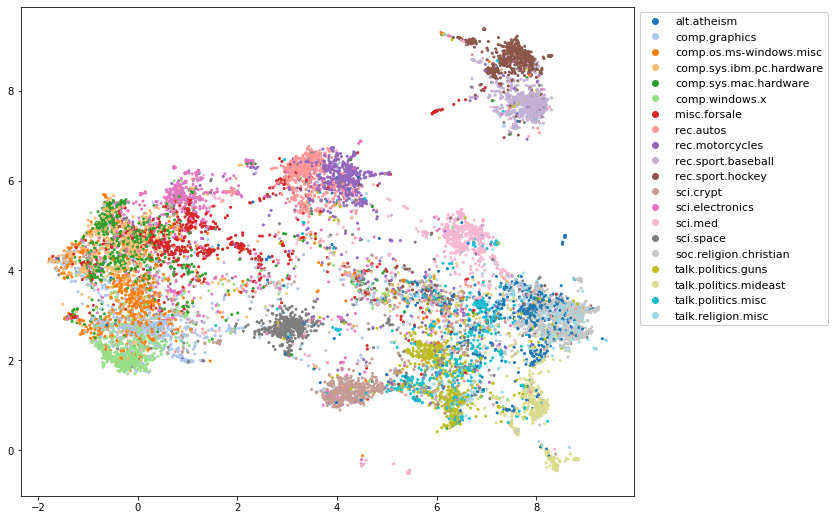
\includegraphics[width=\linewidth]{./assets/orig_umap_train_plot}
      \caption{Original labels}
    \end{subfigure}
    \begin{subfigure}[b]{0.5\linewidth}
      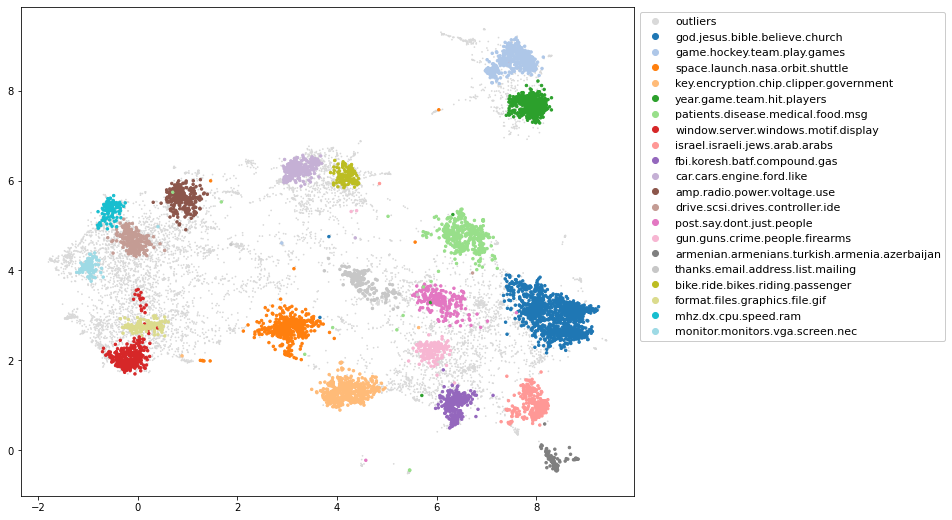
\includegraphics[width=\linewidth]{./assets/top_umap_train_plot}
      \caption{Topic labels}
    \end{subfigure}
  }
  \caption{Comparison between UMAP plots of \textbf{train data} with original and topic labels}
  \label{umap_train_plots}
\end{figure}

\begin{figure}[H]
  \centering
  \resizebox{1\textwidth}{!}{%
    \begin{subfigure}[b]{0.44\linewidth}
      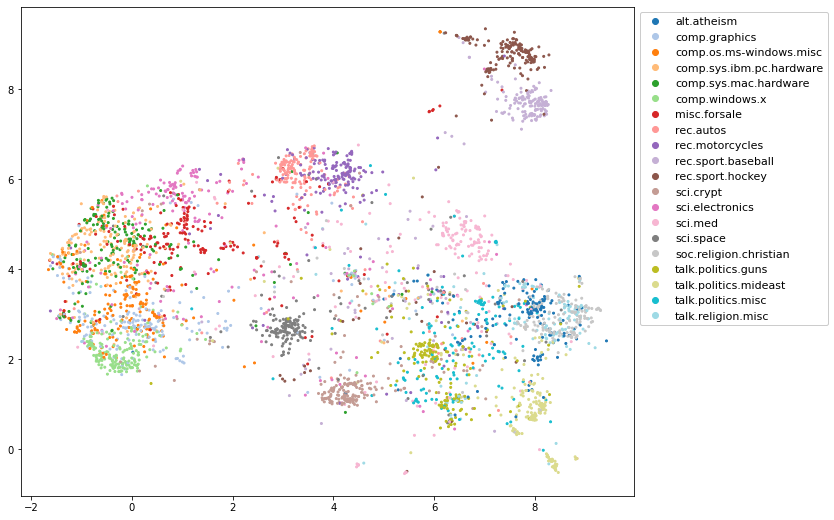
\includegraphics[width=\linewidth]{./assets/orig_umap_test_plot}
      \caption{Original labels}
    \end{subfigure}
    \begin{subfigure}[b]{0.5\linewidth}
      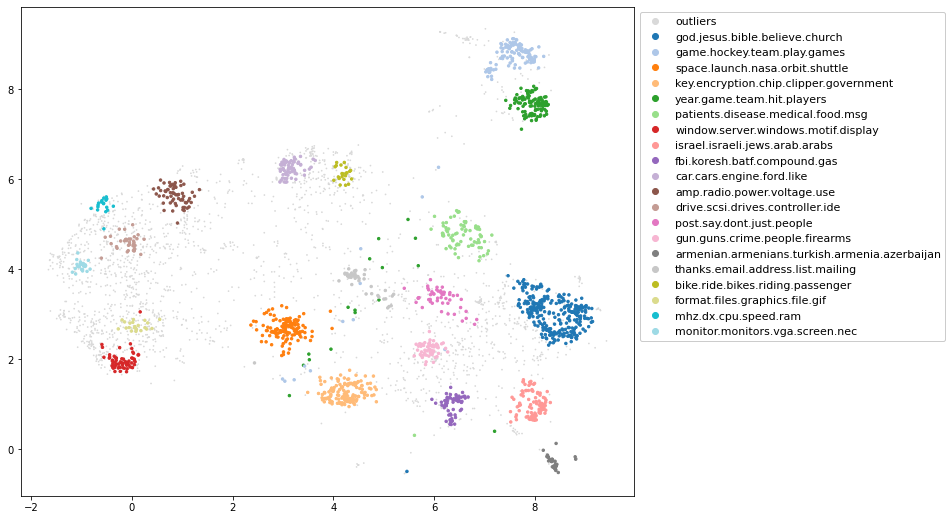
\includegraphics[width=\linewidth]{./assets/top_umap_test_plot}
      \caption{Topic labels}
    \end{subfigure}
  }
  \caption{Comparison between UMAP plots of \textbf{test data} with original and topic labels}
  \label{umap_test_plots}
\end{figure}

\section{Conclusions}
Explain what you have learned and how that influences your next steps. Why does what you discovered matter?

Make sure that you defend your conclusions. (this is conclusions, not opinions!)

\subsection{Future Work}
% Describe your plan of action for the next several weeks of research. Detail the next steps for this team.

%  Zoom in UMAP
We plan to provide a zooming capability on the SOM U-matrix so the user can explore specific regions of the map in detail. There are two ways we have been discussing how to implement this: one possibility would be to allow the user to select a specific unit or group of units on the map and then provide a projection of the underlying documents using either t-SNE \citep{vandermaaten2008} or UMAP \citep{mcinnes2020}; a second possibility would be to allow the user to digitally zoom in on the U-matrix, just like it is done in \citet{kaski1998}. An appealing attribute of this option is the preservation of the landmark labels, which are updated according to the zooming of the map.

% Add a time dimension to the UMAP plot and identify the underlying histories among the articles across time
There's also some discussion on how to integrate release date information on the article's representation. This would allow the documents to be organized not only according to their semantics but also according to their release date. This could also improve the query results as the users are most likely interested in current information. Another feature related to release date would be to relate documents in a timeline, allowing a specific subject to be tracked through time. 

%  Improve the data collection
We would also like to improve the data collection pipeline since we are relying directly on NewsAPI free subscription which has some limitations already described. This would require a substantial effort since web scrapping would most likely be the necessary solution. This approach would provide us with the full article content and would allow us to collect articles as soon as they are released. Multilingual articles could also be collected and integrated into the system by using multilingual embeddings models such as \citet{conneau2019}.

% Add a summarization feature to summarize a set of documents. Add a news feed that allows the user to look at the most recent and relevant news.
Some more ideas to explore consist of: build a single or multi-article summary feature, providing a brief resume of the content of a specific article or a specific SOM unit (collection of articles); add a news article feed based on individual user viewing history. If we plan to expand the application to multiple users, an implicit feedback collaborative filtering \citep{hu2008} approach could be used.

\bibliographystyle{apalike}
\bibliography{bibliography}
\end{document}
